\section{Experiments}
\label{sec:experiments}

\begin{figure}
	\center
	\includegraphics[width=\linewidth]{vect/dataset_ex}
	\caption{\label{fig:dataset} \textbf{Testing sequences examples:} we compare our new localization method on four challenging localization sequences. The number under the query set name indicates the amount of images to localize according to the 1688 reference images.}
\end{figure}

\subsection{Dataset}
\label{subsec:dataset}
	We have tested our new method on the \textit{Oxford Robotcar} public dataset~\cite{Maddern2016}. This is a common dataset used for image based localization~\cite{}(Sattler benchmarking) and loop closure algorithm involving neural netwotks training~\cite{} (day to night for loop closure).
		
\noindent\textbf{Training data.}
	We use dataset temporal redundancy to build our images triplets to train our CNN. We build 400 triplets using three runs acquired at dates: \texttt{2015-05-19, 2015-08-28} and \texttt{2015-11-10}. We selected a different area of city Oxford than the one used for training our networks for validation.
	Depth modality from \textit{Oxford Robotcar} dataset is extracted from the lidar point cloud. When re-projected in the image frame coordinate, it produces a sparse depth map. Deep convolutional neural networks require dense data as input, so we pre-process these sparse modality maps with inpainting algorithm from~\cite{Bevilacqua2017} in order to make them dense.

\noindent\textbf{Testing data.} We propose four testing scenarios on the same spatial area, separate from both training and testing area. Reference dataset is composed of 1688 images taken every 5 meters along a path of 2 km. The fourth query set are:
	\paragraph{Sunny/Overcast} queries have been acquired during a sunny day, whereas the reference data have been acquired when the weather was overcast.
	\paragraph{Long-term} queries have been acquired 7 mouths after the reference images under similar weather conditions.
	\paragraph{Winter/Summer} queries have been acquired during a snowy day.
	\paragraph{Night/Day} queries have been acquired at night, resulting in radical visual changes compare to the reference images.

Query examples are presented in figure~\ref{fig:dataset}.
	
\noindent\textbf{Evaluation metric.} For a given query, reference images are ranked according the cosine similarity score computed over their descriptors. To evaluate the localization performances, we consider two evaluation metrics:
	\setcounter{paragraph}{0}
	\paragraph{Recall @N:} we plot the recall curve regarding the number $N$ of returned candidates, {\it i.e.} a query is considered well localized if one of the top $N$ retrieved images lies inside the $25m$ radius of the ground truth query position.
	\paragraph{Top-1 recall @D} We compute the distance between the top ranked returned database image position and the query ground truth position, and report the percentage of queries located under a threshold D (from 15 to 50 meters), like in~\cite{Zamir2014}. This metric qualifies the precision of the localization system.

\subsection{Implementation details}
\label{subsec:implementation}

For our methods implementation we use Pytorch as deep learning framework, ADAM stochastic gradient descent algorithm for the CNN training with learning rate set to 1e-4, weight decay to 1e-3 and $\lambda$ in triplet loss equations~\ref{eq:triplet_loss},~\ref{eq:depth_triplet_loss},~\ref{eq:cat_triplet_loss} equal to 0.1. Images and depth maps are resized to 224x224 pixels during training and testing.

\noindent\textbf{Encoder architectures.} We test Alexnet (A) and Resnet18 (R) network architectures for features map extraction. We drop the last pooling layer and the fully connected part for both architectures. The size of the final features block is 256*13*13 for Alexnet and 512*7*7 for Resnet. Initial weights are the ones obtained by training the whole network on ImageNet dataset.

We always use Alexnet encoder to extract features from raw depth map, reconstructed depth map, or hallucinated depth map. Indeed the quality of our depth map are very low, we have found that using deeper network do not significantly improves localization results.

\noindent\textbf{Descriptor architectures.} We test the two state of the art image descriptor MAC~\cite{Radenovic2017} and NetVLAD~\cite{Arandjelovic2017}. MAC is a simple global pooling method that takes the maximum of each feature maps from the encoder output. MAC combined with Alexnet encoder produces a 256 dimensions descriptor, whereas combined with Resnet architecture is produce a 512 dimensions descriptor.

NetVLAD is a differentiable and trainable pooling layer that mimic VLAD aggregation method. For all the experiments, we set the number of clusters to 64, resulting on a 16384 dimensions descriptor if it is used with Alexnet features and 32768 dimensions if Resnet features is used instead. The dimension of the final descriptor can be drastically reduced with PCA-whitening post-processing.

Finally, both MAC and NetVLAD descriptors are $L_{2}$ normalized.

\noindent\textbf{Truncated Resnet.} NetVLAD can be view as a pooling method that acts on local deep features densely extracted from the input image. We found that NetVLAD descriptor combined with Resnet architecture do not perform well. We argue that the spatial resolution of the features block obtained with Resnet encoder is too low compare to other architecture (for instance 13*13 for Alexnet compare to 7*7 for Resnet for an 224*224 input image). We propose a truncated version of Resnet encoder (Rt) by drooping layers after the 13th convolutional layer, thus obtaining a features block with greater spatial resolution of size 256*14*14. Recall results on the \textit{Sunny/Overcast} query set for both architectures are presented in figure~\ref{fig:trunc_resnet}. As the truncated version of Resnet encoder clearly dominated the full one, we use the truncated version for the following experiments.

\subsection{Results}
\label{subsec:results}

\begin{figure}
	\center
	\begin{minipage}{0.49\linewidth}
		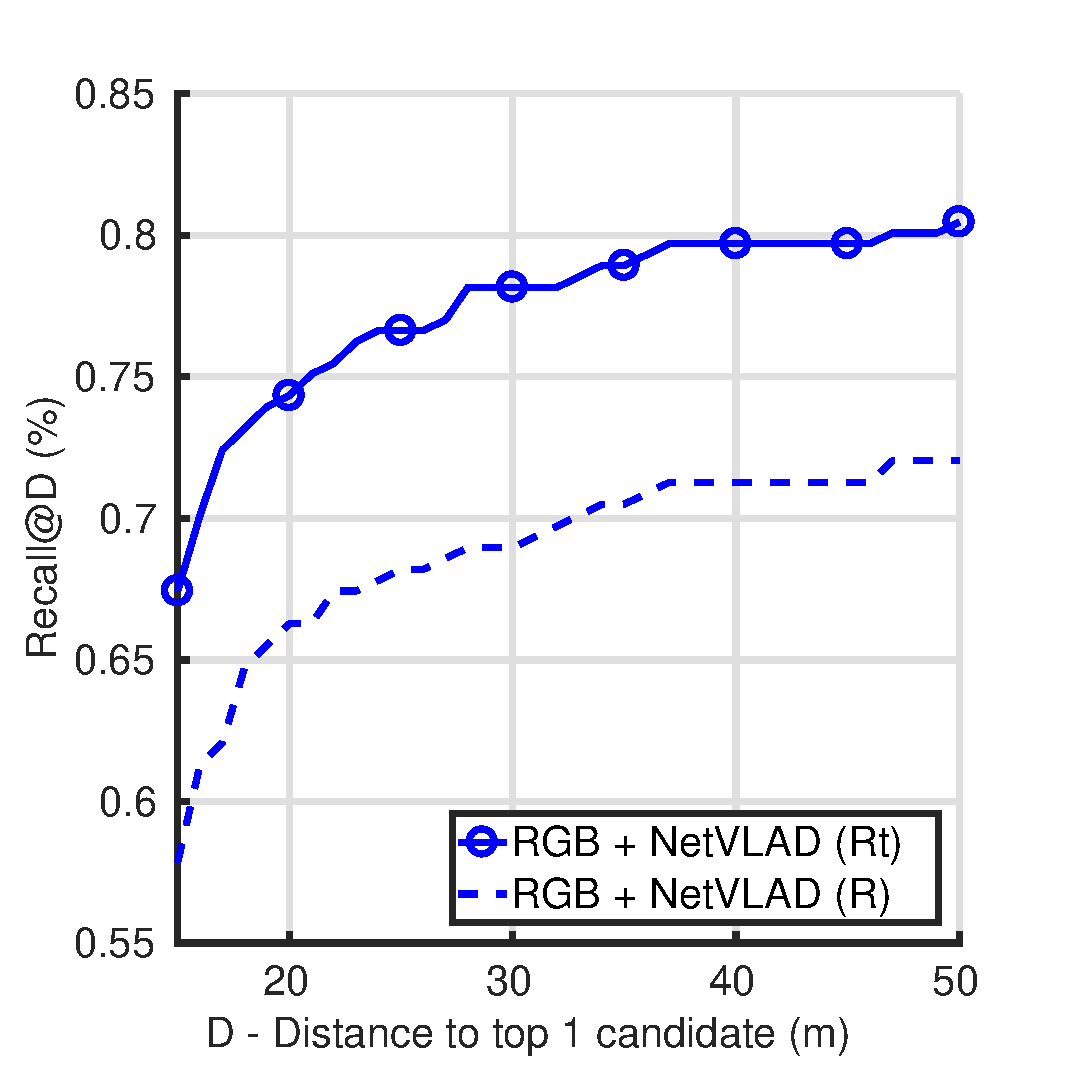
\includegraphics[width=\linewidth]{plot/fig/rgb_r_trunc_distance}	
	\end{minipage}
	\begin{minipage}{0.49\linewidth}
		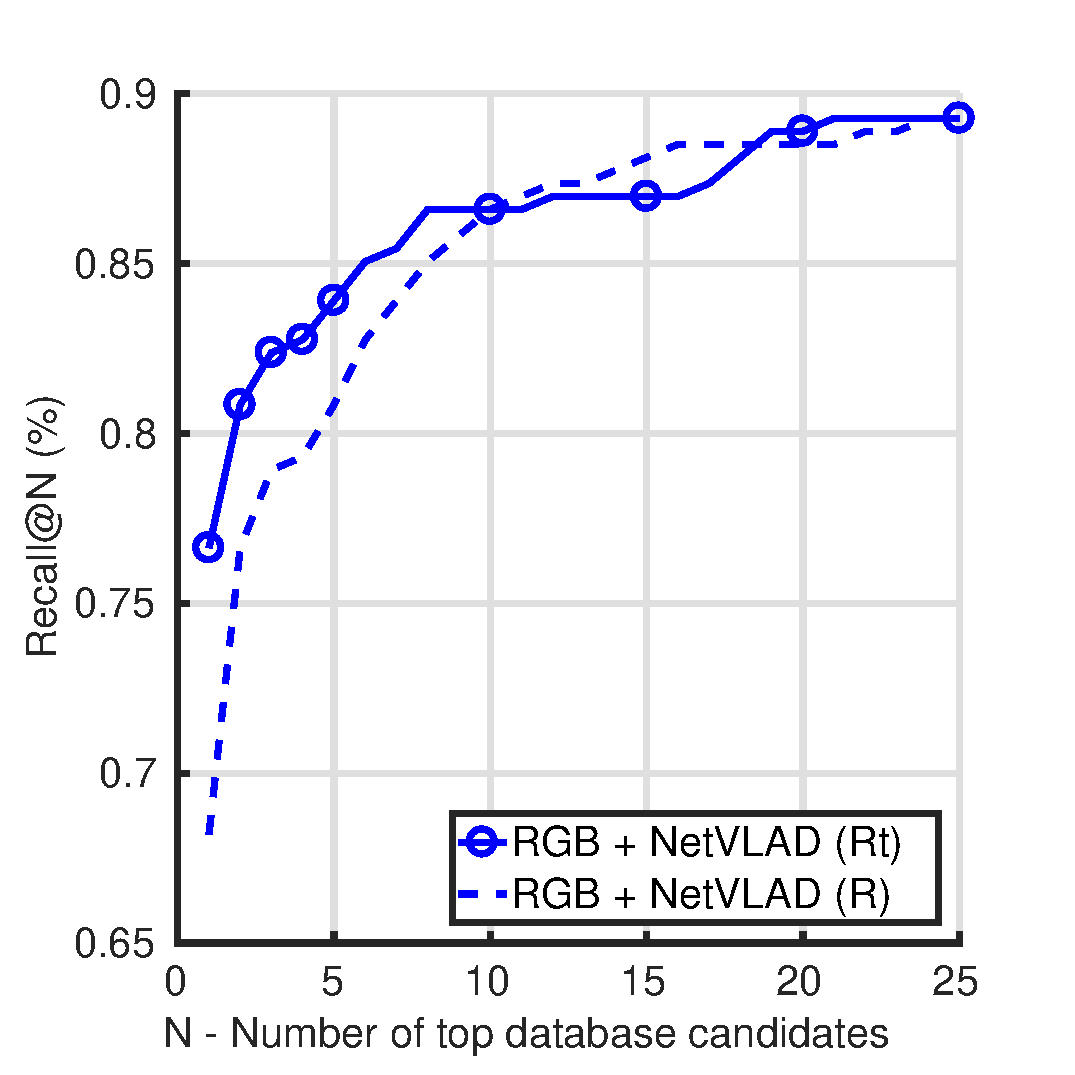
\includegraphics[width=\linewidth]{plot/fig/rgb_r_trunc_recall}	
	\end{minipage}
	\caption{\label{fig:trunc_resnet} \textbf{Truncated Resnet + NetVLAD}}
\end{figure}

\begin{figure*}
	\center
	\begin{minipage}{0.14\linewidth}
		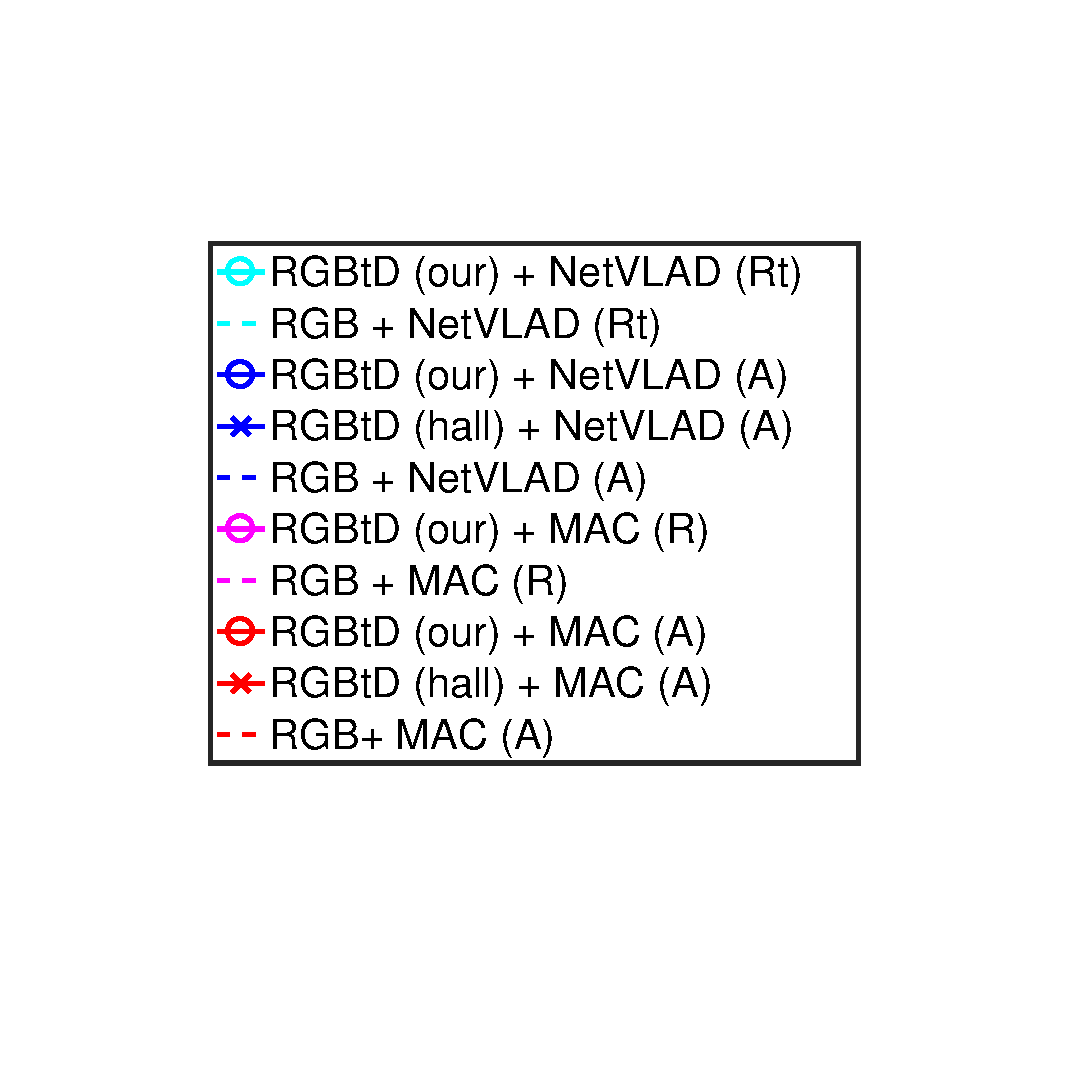
\includegraphics[trim={150 170 210 255},clip,width=\linewidth]{plot/fig/legend}	
	\end{minipage}
	\begin{minipage}{0.85\linewidth}
	
	\begin{minipage}{0.49\linewidth}		
		\center
		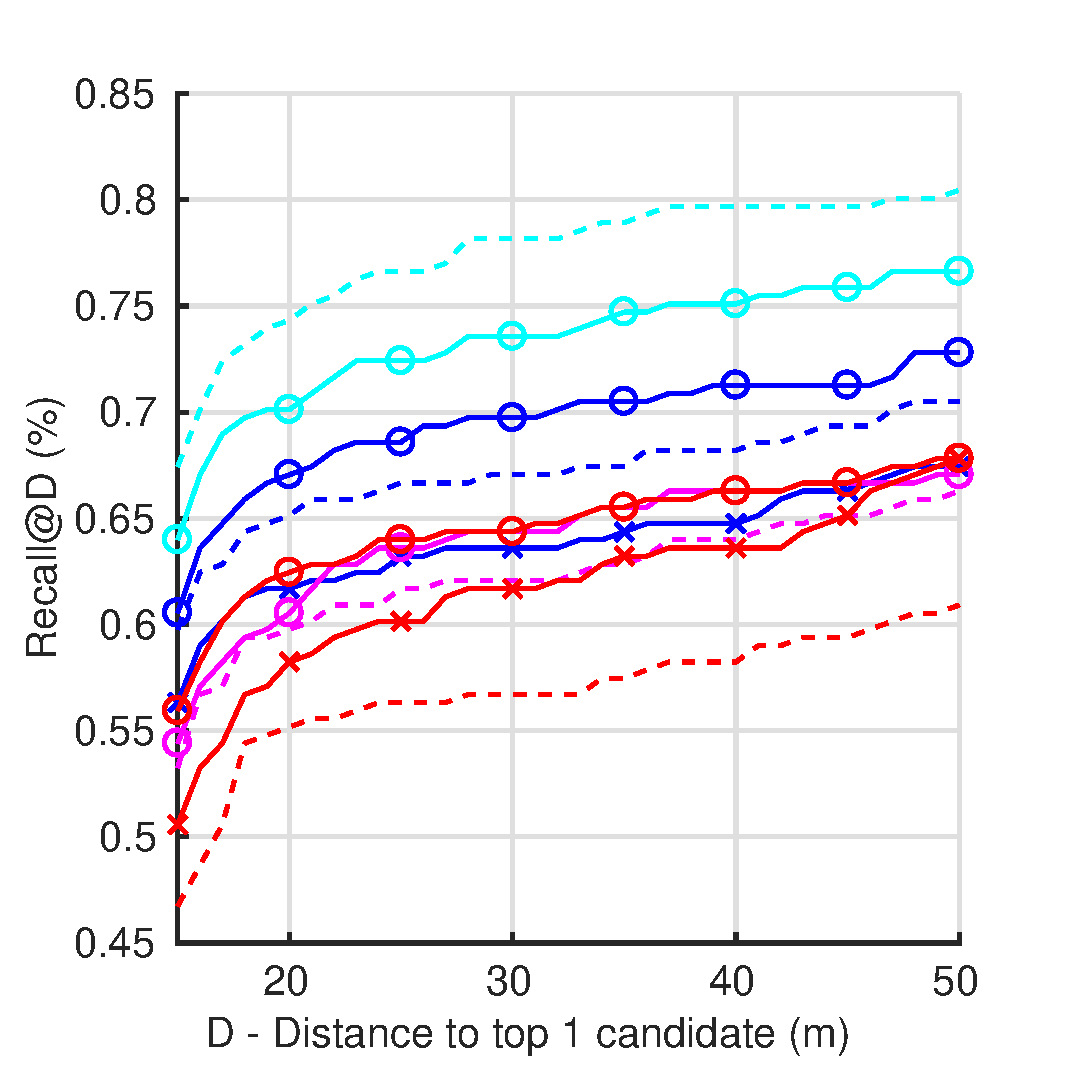
\includegraphics[width=0.49\linewidth]{plot/fig/sun_distance}	
		\includegraphics[width=0.49\linewidth]{plot/fig/sun_recall}
		
		{\scriptsize a) Sunny/Overcast}
	\end{minipage}
	\begin{minipage}{0.49\linewidth}
		\center
		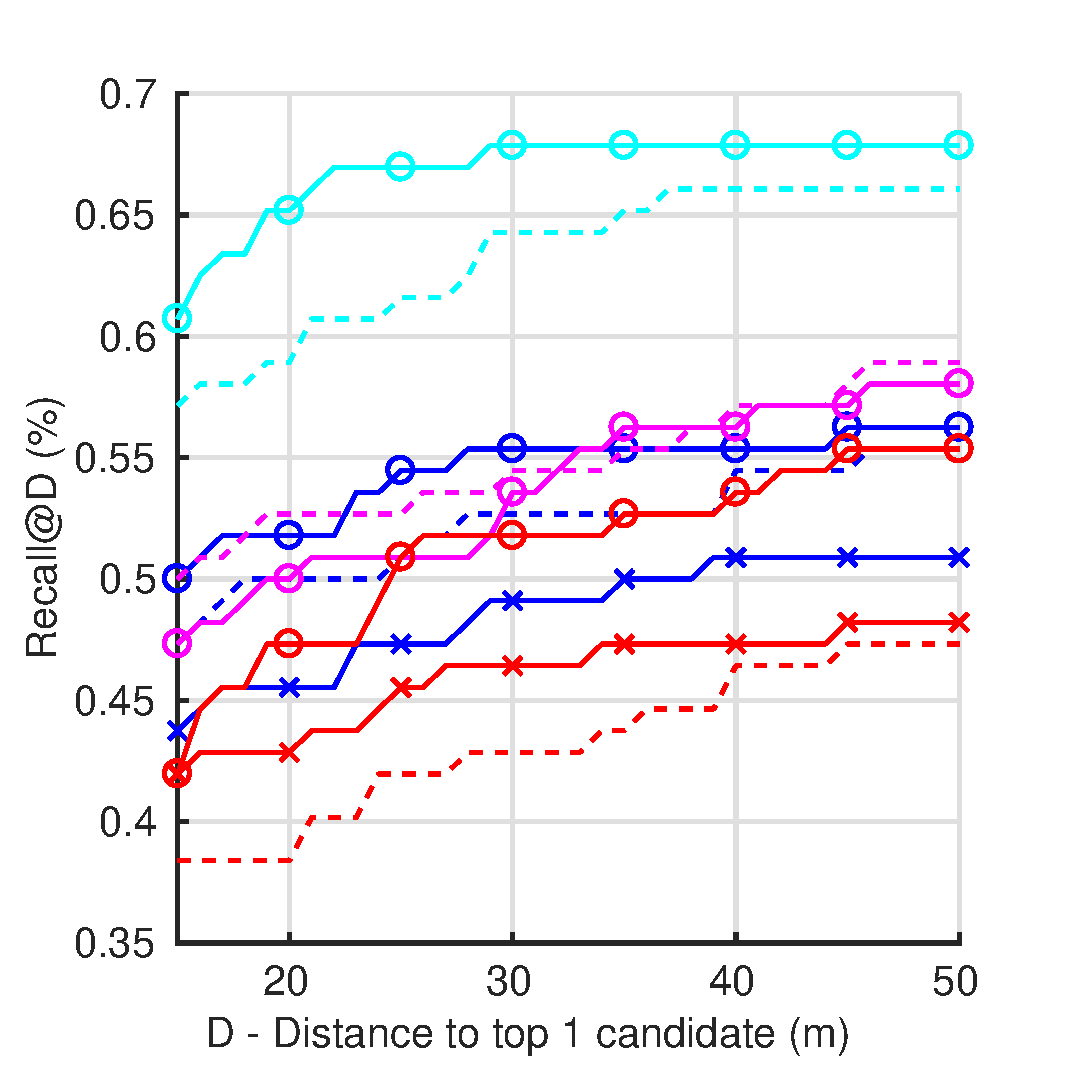
\includegraphics[width=0.49\linewidth]{plot/fig/snow_distance}	
		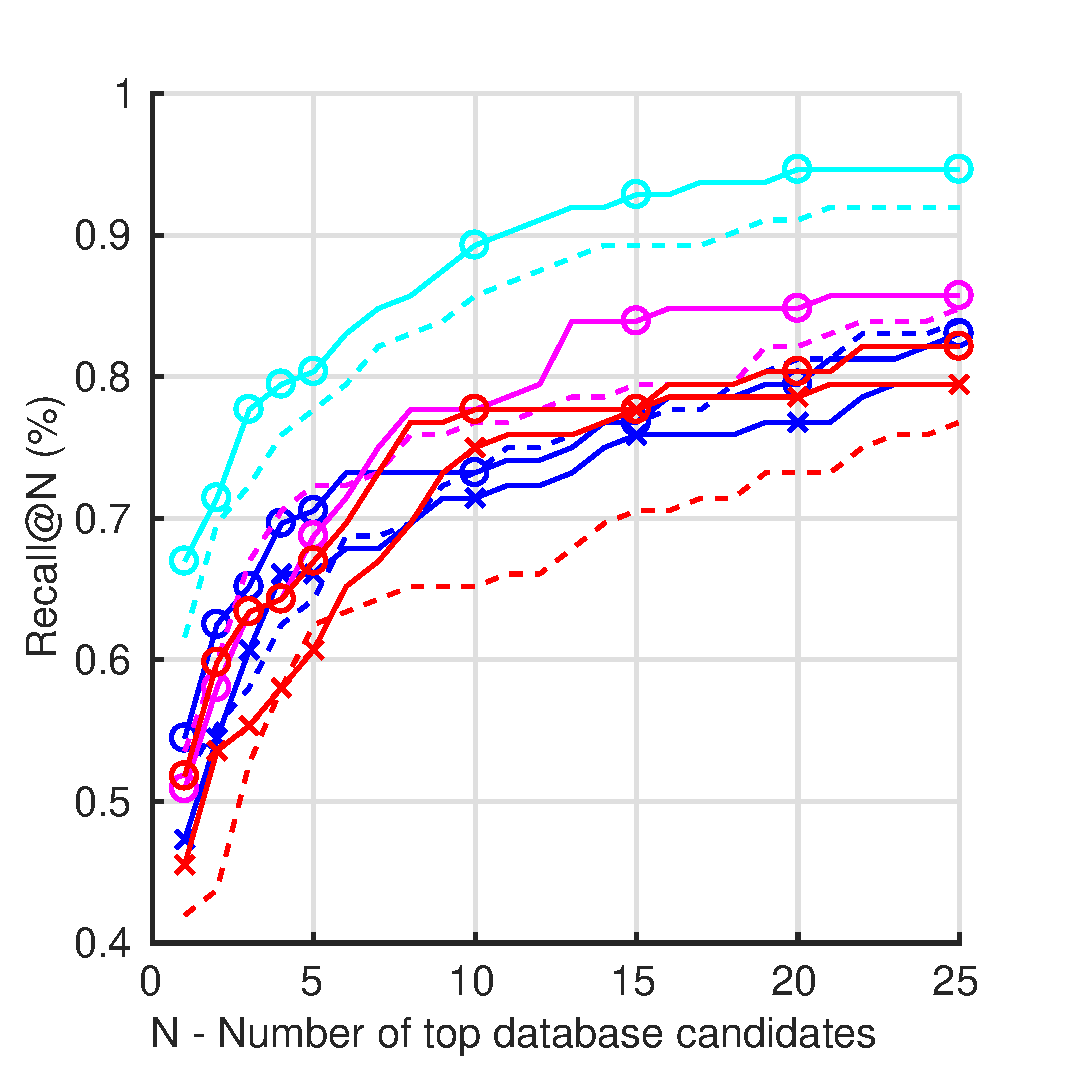
\includegraphics[width=0.49\linewidth]{plot/fig/snow_recall}
		
		{\scriptsize b) Winter/Summer}
	\end{minipage}
	
	\begin{minipage}{0.49\linewidth}
		\center
		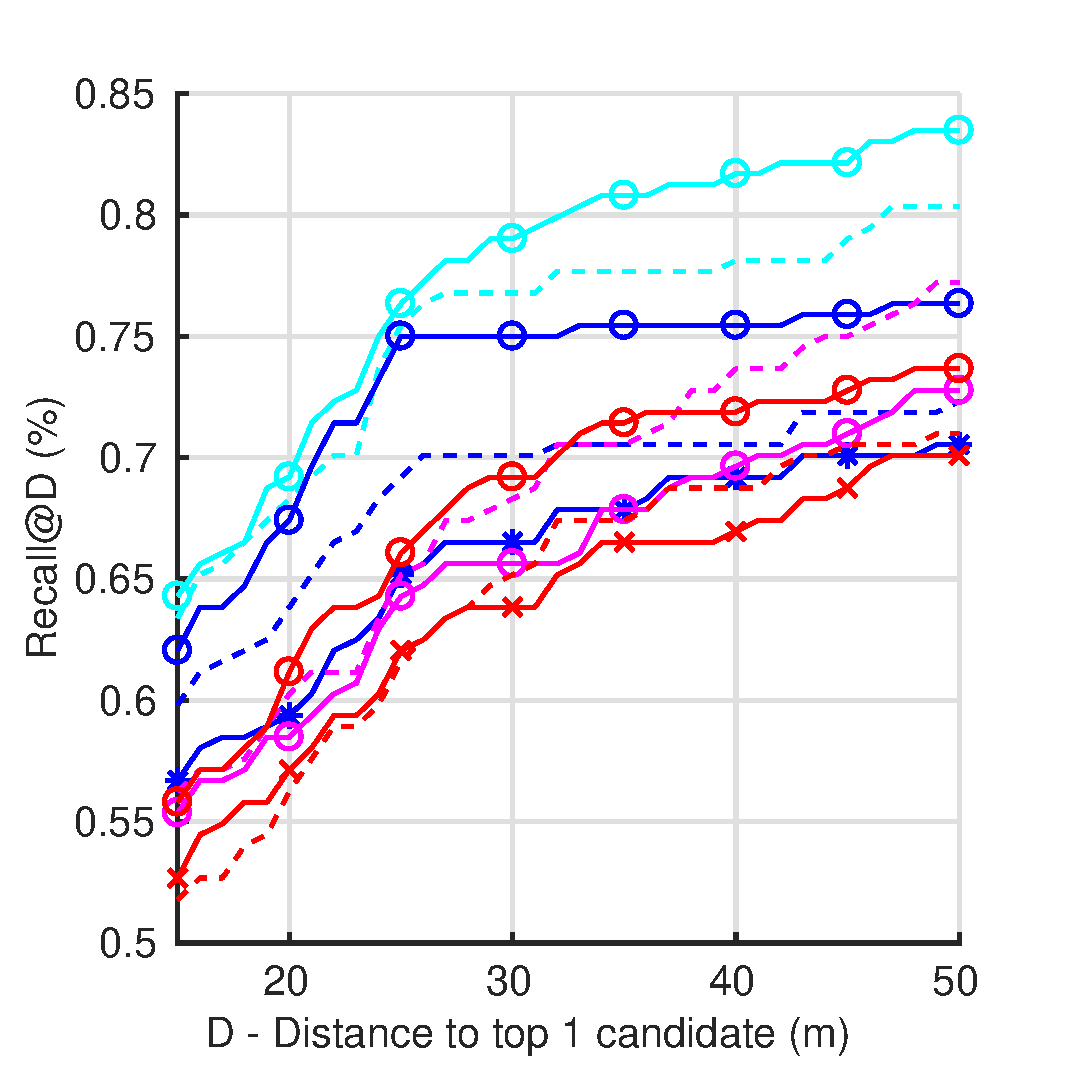
\includegraphics[width=0.49\linewidth]{plot/fig/lt_distance}	
		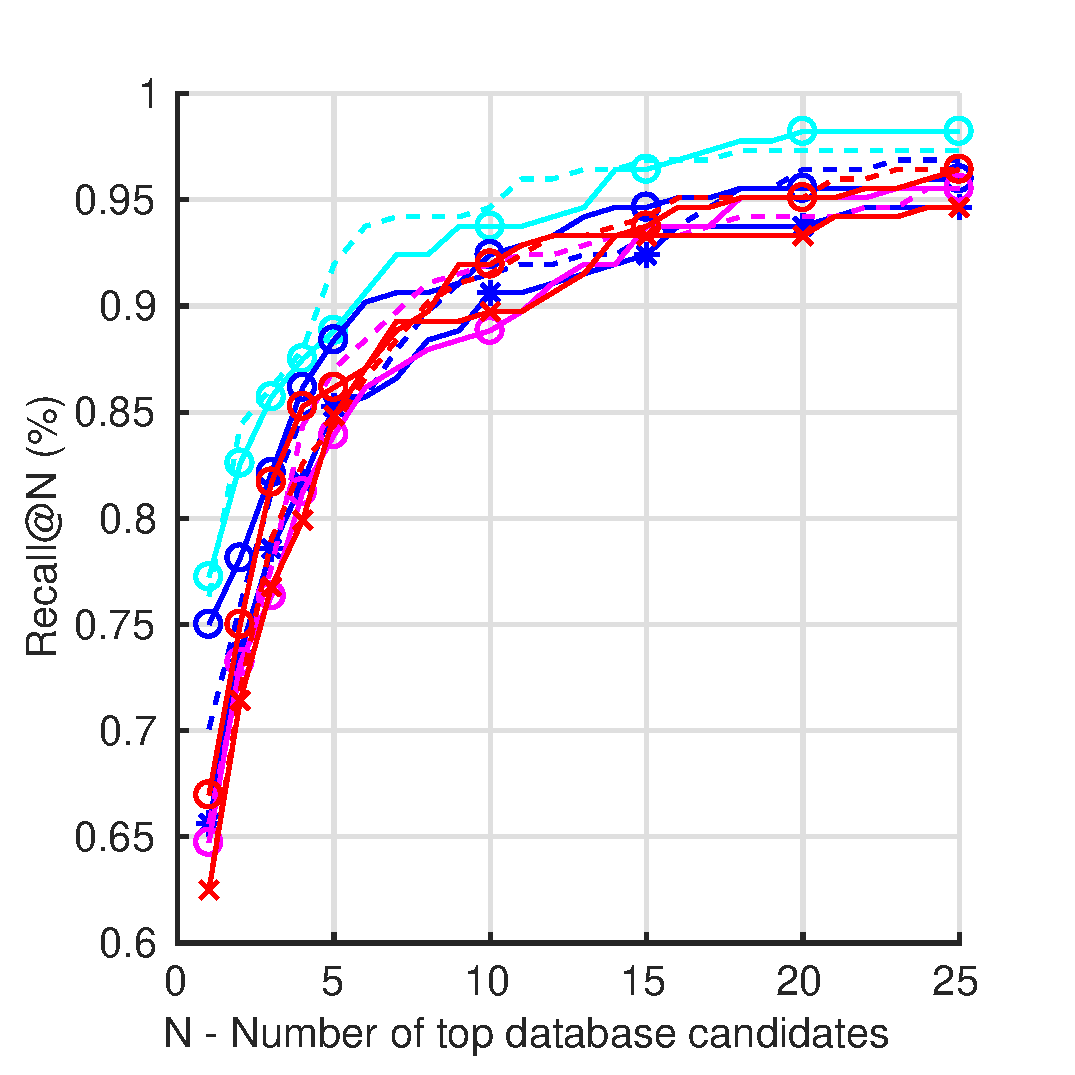
\includegraphics[width=0.49\linewidth]{plot/fig/lt_recall}

		{\scriptsize c) Long-term}		
	\end{minipage}
	\begin{minipage}{0.49\linewidth}
		\center	
		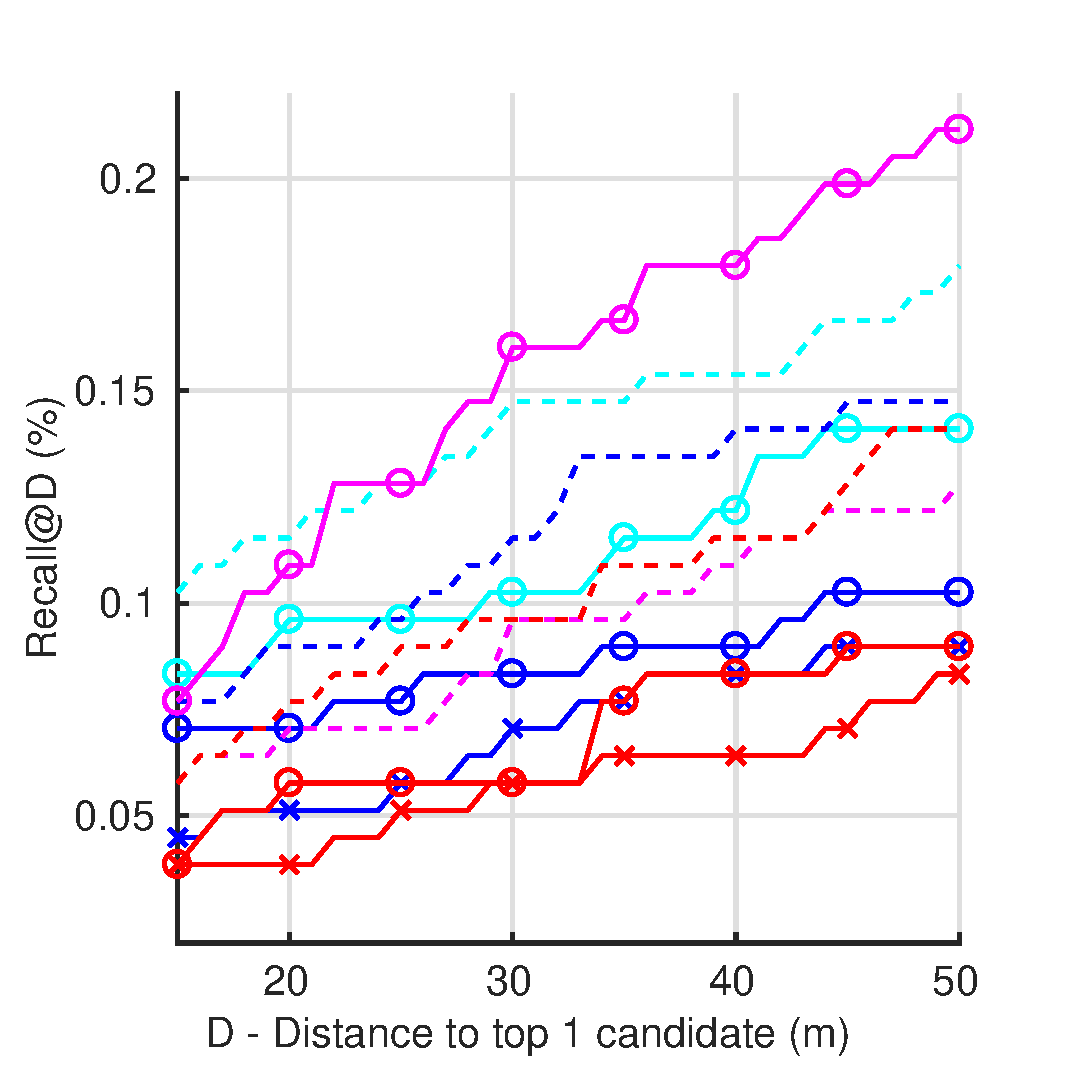
\includegraphics[width=0.49\linewidth]{plot/fig/night_distance}	
		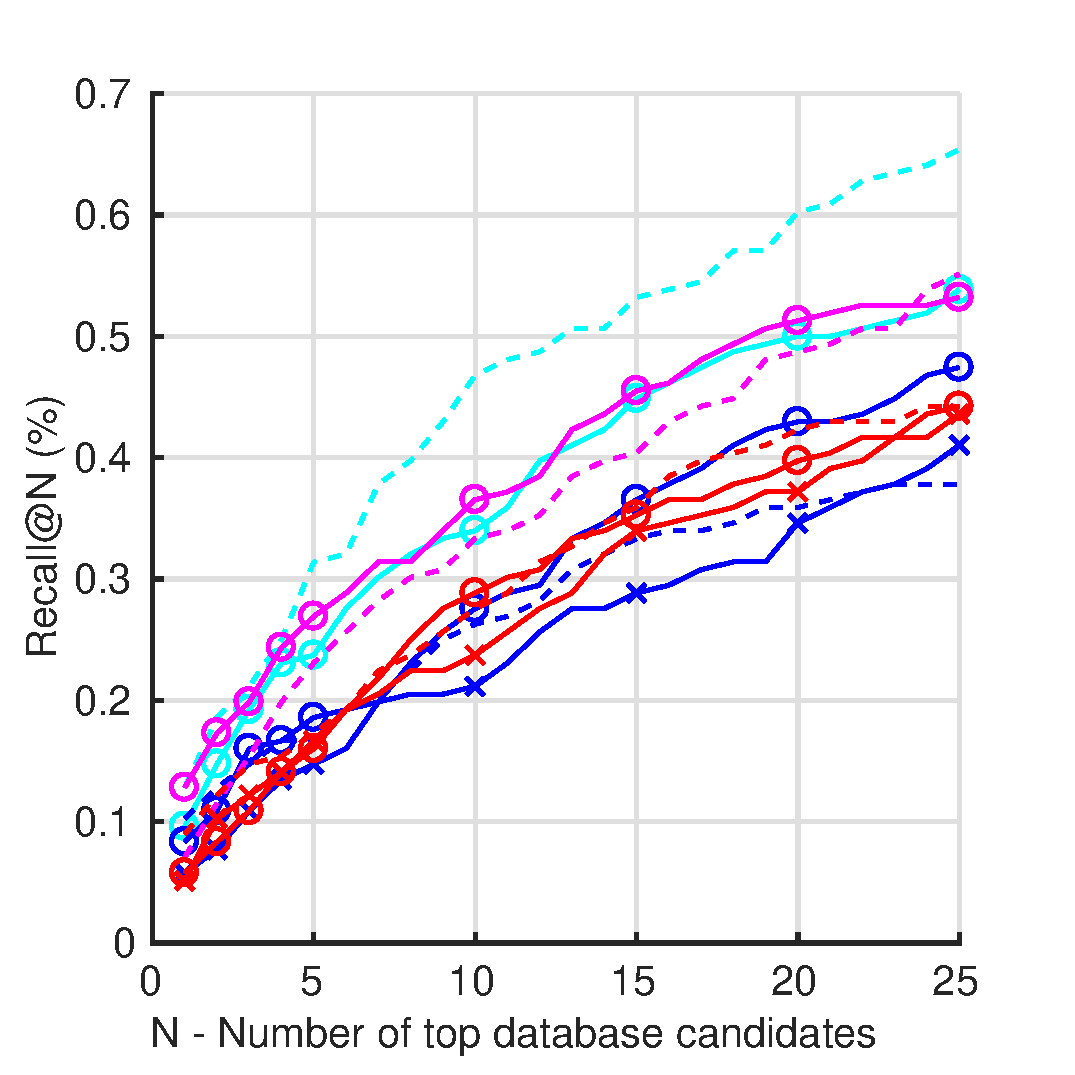
\includegraphics[width=0.49\linewidth]{plot/fig/night_recall}
	
		{\scriptsize d) Night/Day}
	\end{minipage}
	
	\end{minipage}

	\caption{\label{fig:results} \textbf{Results}}
\end{figure*}

Short-terme localisation

Long-terme localisation

Night to day localisation

Winter to summer localisation
